\documentclass{beamer}
\usepackage{amsfonts,amsmath,oldgerm}
\usetheme{sintef}
\usepackage{multicol}

\usepackage{longtable}
\newcommand{\testcolor}[1]{\colorbox{#1}{\textcolor{#1}{test}}~\texttt{#1}}

\usefonttheme[onlymath]{serif}

\titlebackground*{assets/background}

\newcommand{\hrefcol}[2]{\textcolor{cyan}{\href{#1}{#2}}}

\title{Computer Architecture and Operating System}
\subtitle{HackOSsim Project}
\course{Master's Degree in Cybersecurity}
\author{
    \href{mailto:user3@studenti.polito.it}{Giuseppe Famà}\IDnumber{54321},
    \href{mailto:user2@studenti.polito.it}{Youssef Rachid Grib}\IDnumber{67890},
    \href{mailto:vincenzo.longo@studenti.polito.it}{Vincenzo Longo}\IDnumber{328843}
}
\date{September 20, 2024}

\begin{document}
\maketitle

\section{Introduction}

\begin{frame}{The Goal of this Project}

The goal of this project consists in analysing and using the real time OS \hrefcol{https://www.freertos.org/}{FreeRTOS} exploiting the \hrefcol{https://www.qemu.org/}{QEMU}\footnote{It allows to virtualize several types of hardware architecture.} simulator. In the following you find a detailed tutorial for the \textbf{installation} and usage procedures and some \textbf{practical examples} and \textbf{new implementations} to demonstrate the functionality of the operating system.

\end{frame}

\section{Environment Setup}
\begin{frame}{Installation}
    To setup the environment the following steps has been followed:
    \begin{itemize}
        \item Downloading the \texttt{FreRTOS} repository;
        \item Downloading of \texttt{QEMU} emulator;
        \item Setup of other tools:
        \begin{itemize}
            \item \texttt{ARM GNU Toolchain};
            \item \texttt{CMake};
            \item \texttt{Make};
        \end{itemize}
        \item Finally we proceed with the environment configuration;
    \end{itemize}
\end{frame}

\begin{frame}{Intro to the Demo Applications}

\vfill % Creates vertical space before the content
\centering
\begin{columns}[c] % Center the columns vertically
    \begin{column}{0.5\textwidth}
        In this project, each single demo application can be selected by properly setting the \texttt{mainCREATE\_SIMPLE\_DEMO} value in the \texttt{main.c} file.
    \end{column}

    \begin{column}{0.4\textwidth}
        \begin{figure}
            \centering
            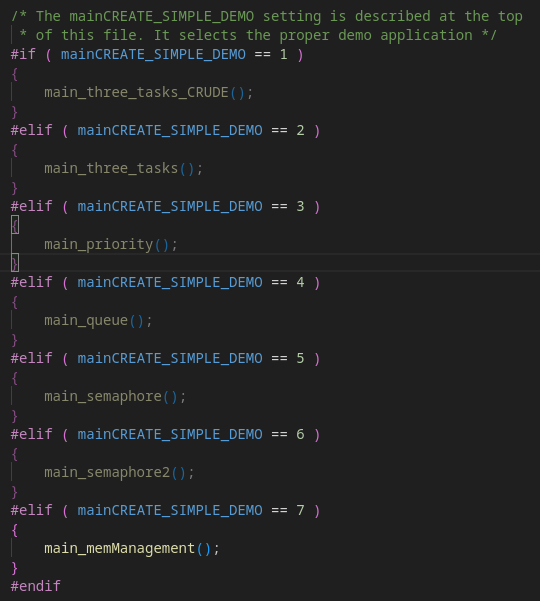
\includegraphics[width=\linewidth]{img/mainCREATE_SIMPLE_DEMO.png}
            \label{fig:mainCREATE_SIMPLE_DEMO}
        \end{figure}
    \end{column}
\end{columns}

\end{frame}


\section{Task Management}
\begin{frame}{Demo Applications}
    \begin{itemize}
        \item \textbf{main\_three\_task\_CRUDE.c}
        \begin{itemize}
            \item Tasks with the \textbf{SAME priority}.
            \item Each task implements the same function that \textbf{prints a message}.
            \item After printing the message, the task enters in a \textbf{loop} whose the unique functionality is the implementation of a \textbf{CRUDE delay}, i.e., which does not move the task in the \texttt{waiting list}.
        \end{itemize}
        \item \textbf{main\_three\_task.c}
        \begin{itemize}
            \item \textbf{NO CRUDE DELAY}!
            \item API function \texttt{VTaskDelayUntil()}.
            \item This function just moves the task in the blocked state, making room for tasks in the ready state.
        \end{itemize}
        \item \textbf{main\_priority.c}
        \begin{itemize}
            \item More advanced example to show how \textbf{FreeRTOS scheduler} works.
            \item One of the two tasks has dynamic priority.
        \end{itemize}
    \end{itemize}
\end{frame}

\begin{frame}{Process Flow - main\_three\_task\_CRUDE.c}

\vfill
\centering
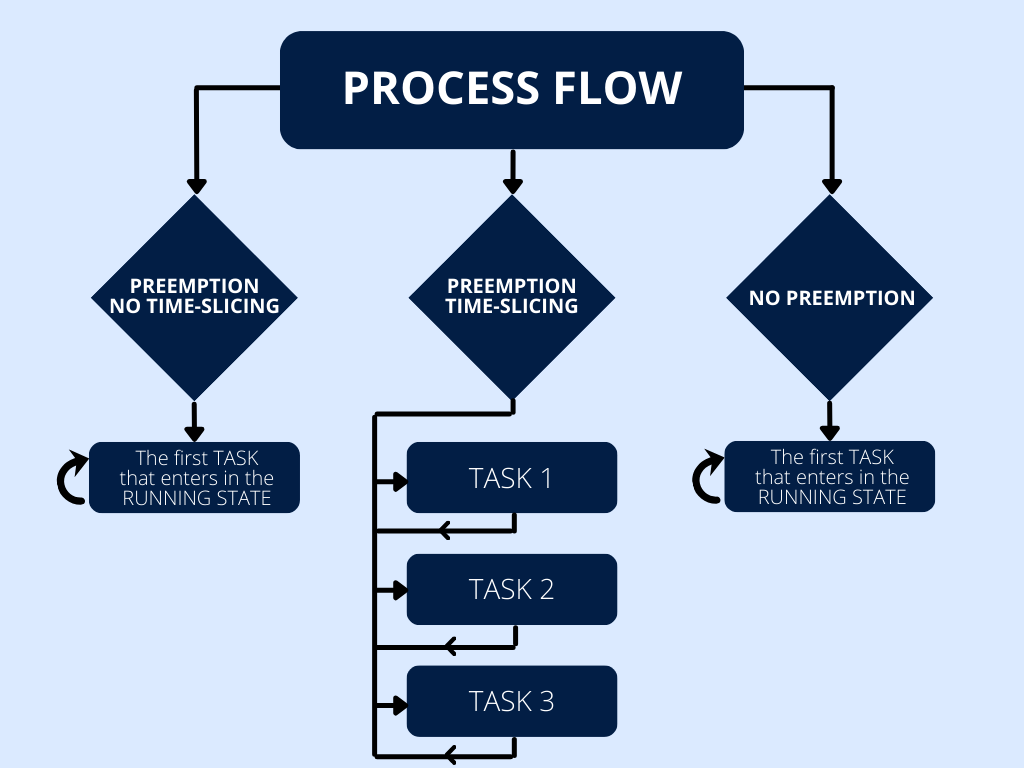
\includegraphics[width=0.65\linewidth]{img/three_tasks_CRUDE.png} 
\vfill
    
\end{frame}

\begin{frame}{Process Flow - main\_three\_task.c}

\vfill
\centering
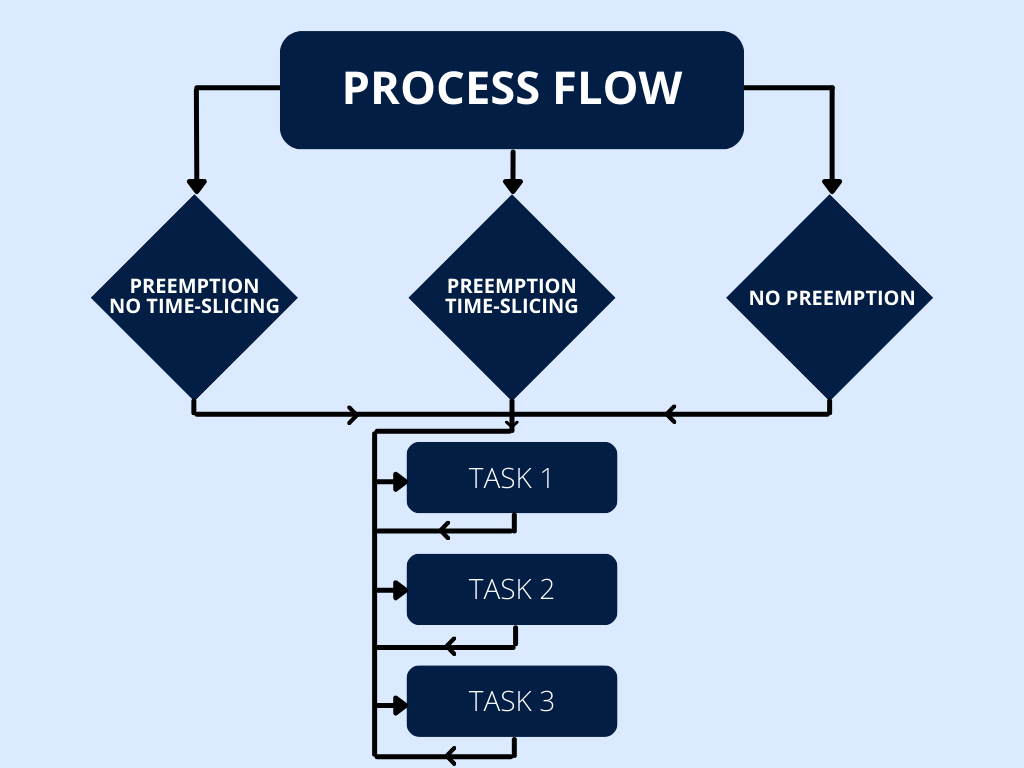
\includegraphics[width=0.65\linewidth]{img/three_tasks.png} 
\vfill
    
\end{frame}

\begin{frame}{Process Flow - main\_priority.c}

\vfill
\centering
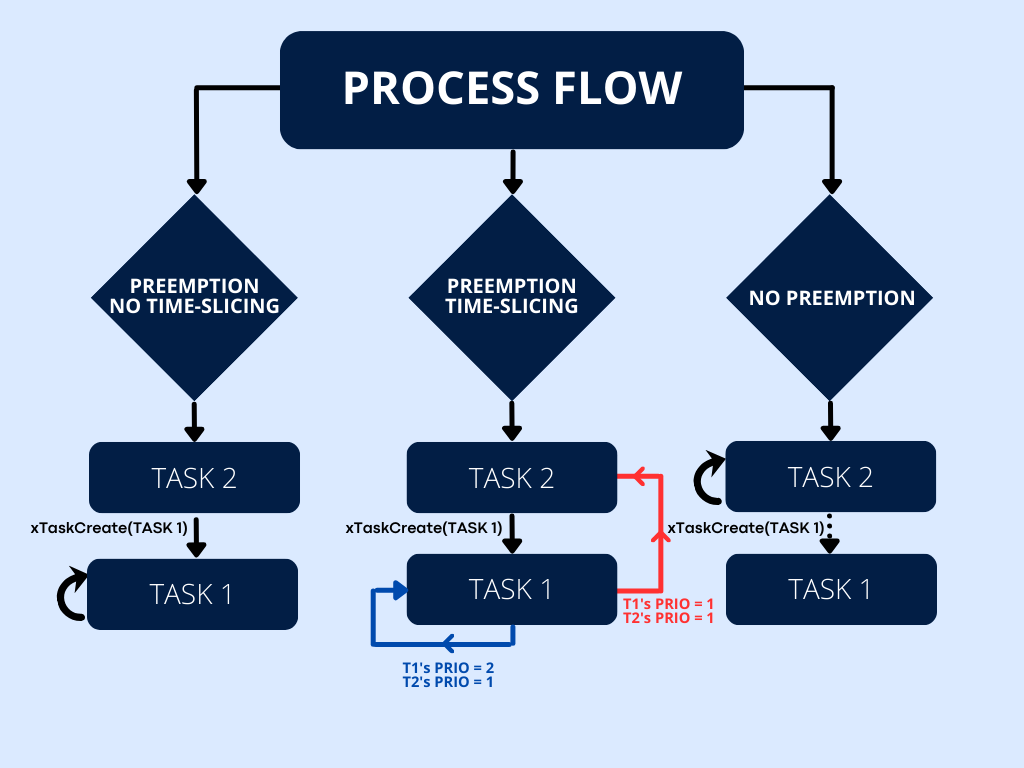
\includegraphics[width=0.65\linewidth]{img/dynamic_priority.png} 
\vfill
    
\end{frame}

\section{Queue and Task Synchronization}
\begin{frame}{Demo Applications}
        \begin{itemize}
        \item \textbf{main\_queue.c}
        \begin{itemize}
            \item Three \textbf{PRODUCERS} and one \textbf{CONSUMER} (\textbf{highest priority}).
            \item The \textbf{CONSUMER} is blocked when the queue is empty, unblocking the \textbf{PRODUCERS}.
        \end{itemize}
        \item \textbf{main\_semaphore.c}
        \begin{itemize}
            \item Three \textbf{PRODUCERS} and one \textbf{CONSUMER} handled with \textbf{two binary semaphores}.
            \item At the beginning the \textbf{PRODUCERS} enter in the critical section \textbf{until the queue is fulfilled}.
            \item Then the \textbf{CONSUMER} reads out all the data.
            \item \textbf{Any priority can be used}! Semaphores synchronize the tasks.
        \end{itemize}
        \item \textbf{main\_semaphore2.c}
        \begin{itemize}
            \item Three \textbf{PRODUCERS} and one \textbf{CONSUMER} handled with \textbf{four semaphores} (3 binary and 1 counting).
            \item Each \textbf{PRODUCER} inserts its value and unblocks the next task.
            \item Once all the \textbf{PRODUCERS} inserted their values, the \textbf{CONSUMER} reads out all the items, then unblocks the first \textbf{PRODUCER}.
            \item \textbf{Any priority can be used}! Semaphores synchronize the tasks.
        \end{itemize}
    \end{itemize}
\end{frame}

\begin{frame}{Precedence Diagrams - main\_queue.c}

\vfill
\centering
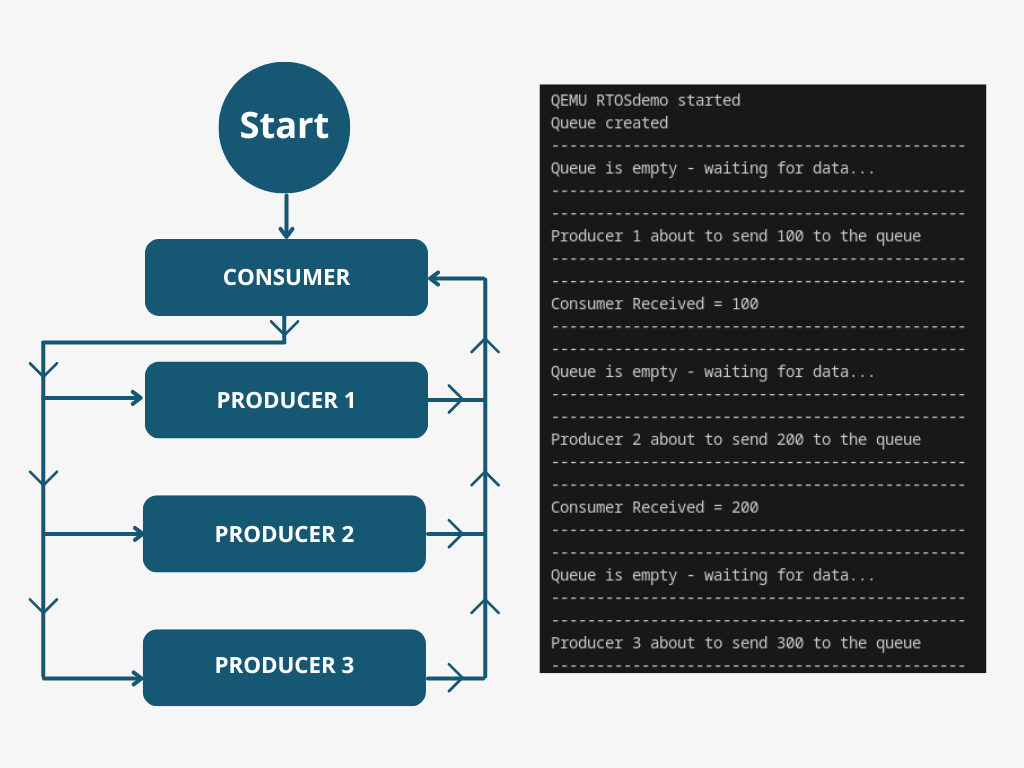
\includegraphics[width=0.7\linewidth]{img/main_queue.png} 
\vfill
    
\end{frame}

\begin{frame}{Precedence Diagrams - main\_semaphore.c}

\vfill
\centering
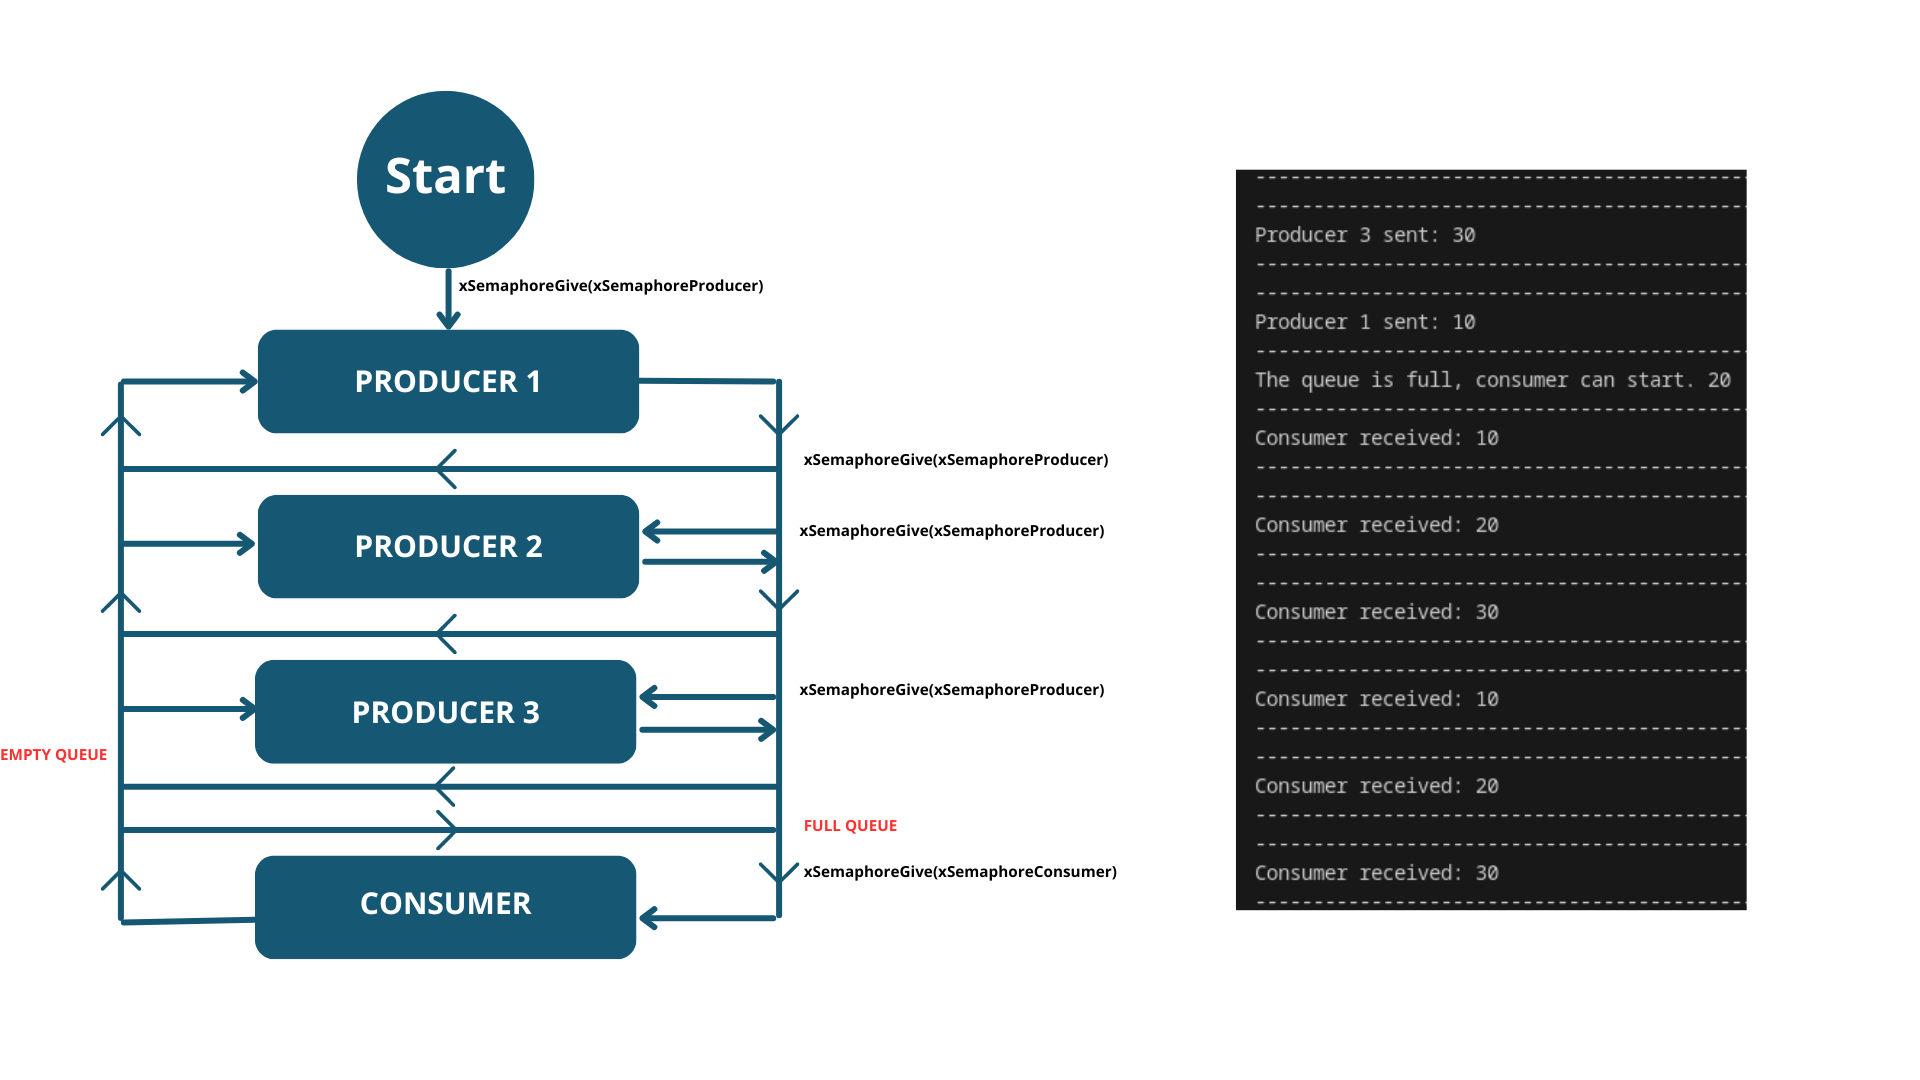
\includegraphics[width=0.95\linewidth]{img/precedence_diagram_semaphore1.png} 
\vfill
    
\end{frame}

\begin{frame}{Precedence Diagrams - main\_semaphore2.c}

\vfill
\centering
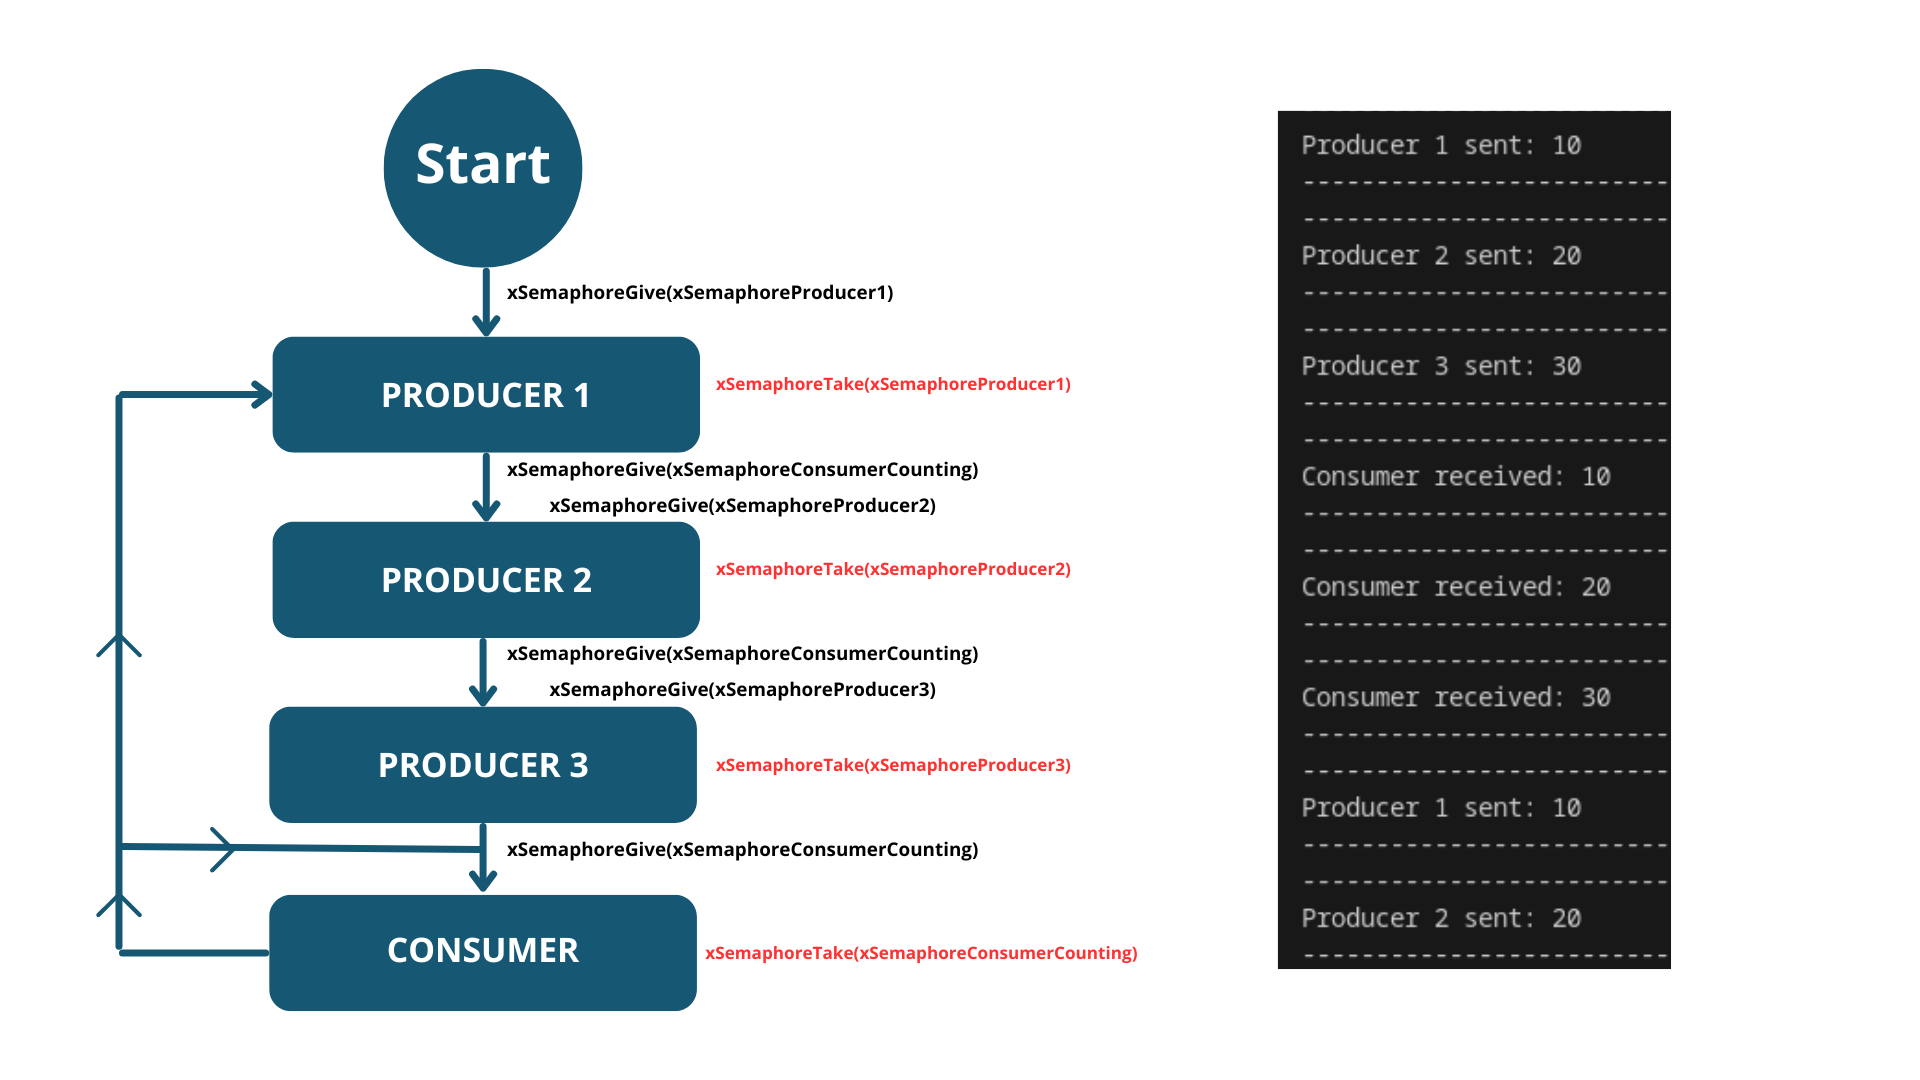
\includegraphics[width=0.95\linewidth]{img/precedence_diagram_semaphore2.png} 
\vfill
    
\end{frame}




\section{Memory Management}
\begin{frame}{Implementation}

To better analyze the Memory Management the provided \texttt{heap\_4.c} file was revised to implement:
\begin{itemize}
    \item \textbf{Best-Fit}: The process is allocated in smallest available memory block that is large enough for the process.  
    \item \textbf{Worst-Fit}: The process is allocated in the largest available memory block.
    \item \textbf{First-Fit}: The process is allocated in the first available memory block.
\end{itemize}

    
\end{frame}

\begin{frame}{Perfomance Evaluation}
The main perform the following steps:
\begin{multicols}{2} % Inizia l'ambiente a due colonne
\begin{enumerate}
    \item \textbf{Allocates 1000 bytes}
    \item \textbf{Allocates 1000 bytes}
    \item \textbf{Allocates 1500 bytes}
    \item \textbf{Allocates 100 bytes}
    \item \textbf{Allocates 100 bytes}
    \item \textbf{Allocates 100 bytes}
    \item \textbf{Allocates 100 bytes}
    \item \textbf{De-allocates 1000 bytes (second block)}
    \item \textbf{De-allocates 100 bytes (fourth block)}
    \item \textbf{De-allocates 100 bytes (fifth block)}
    \item \textbf{De-allocates 100 bytes (sixth block)}
    \item \textbf{Allocates 300 bytes}
    \item \textbf{Allocates 1000 bytes}
    \item \textbf{Creates a task (TASK 1)}
\end{enumerate}
\end{multicols}
\end{frame}

\begin{frame}{First-Fit and Worst-Fit output 1/2}
   \vfill
    \centering
    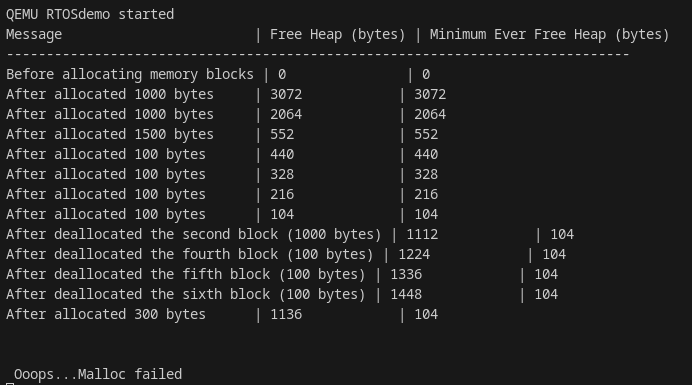
\includegraphics[width=0.8\linewidth]{img/first-worst-fit_output.png} 
    \vfill 
\end{frame}

\begin{frame}{First-Fit and Worst-Fit output 2/2}
   \vfill
    \centering
    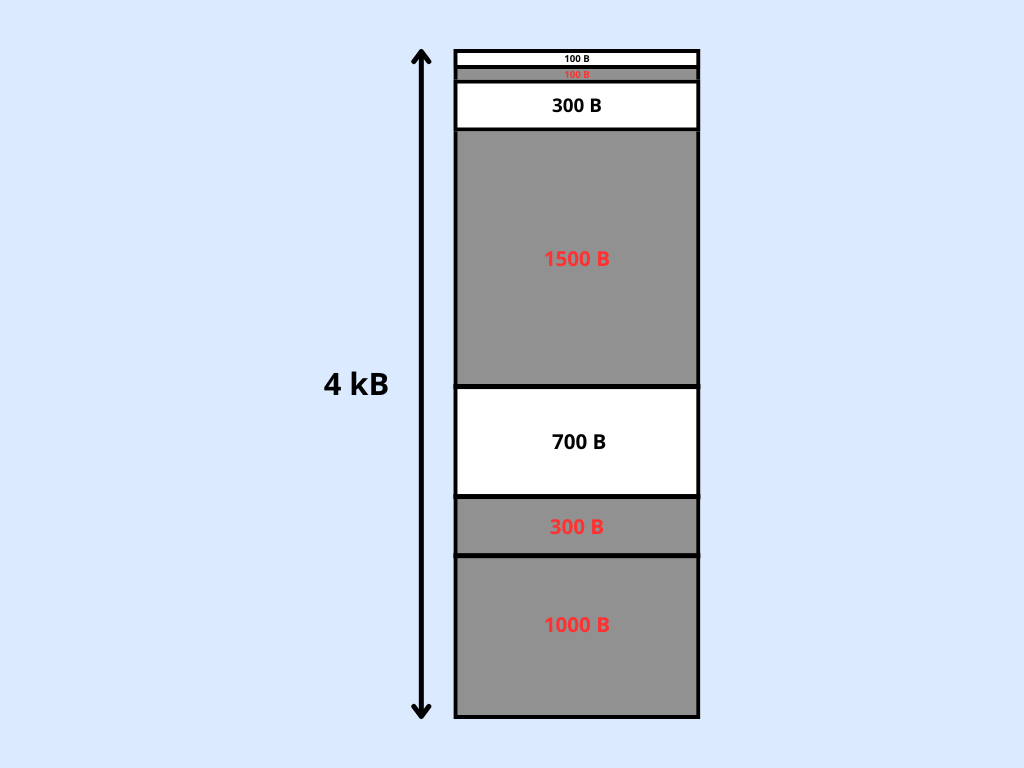
\includegraphics[width=0.65\linewidth]{img/first-worst.png} 
    \vfill 
\end{frame}

\begin{frame}{Best-Fit output 1/2}
    \vfill
    \centering
    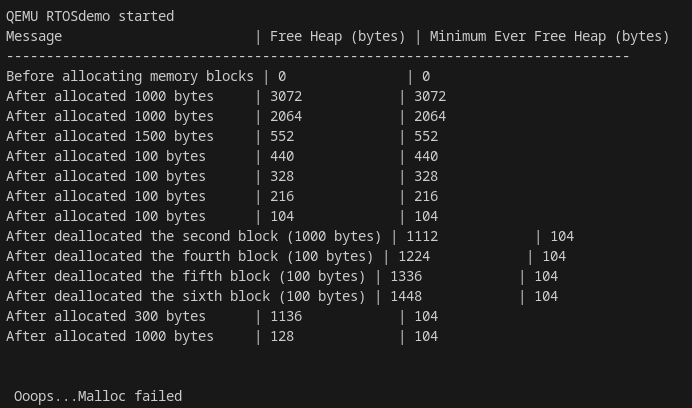
\includegraphics[width=0.8\linewidth]{img/best-fit_output.png} 
    \vfill 
\end{frame}

\begin{frame}{Best-Fit output 2/2}
    \vfill
    \centering
    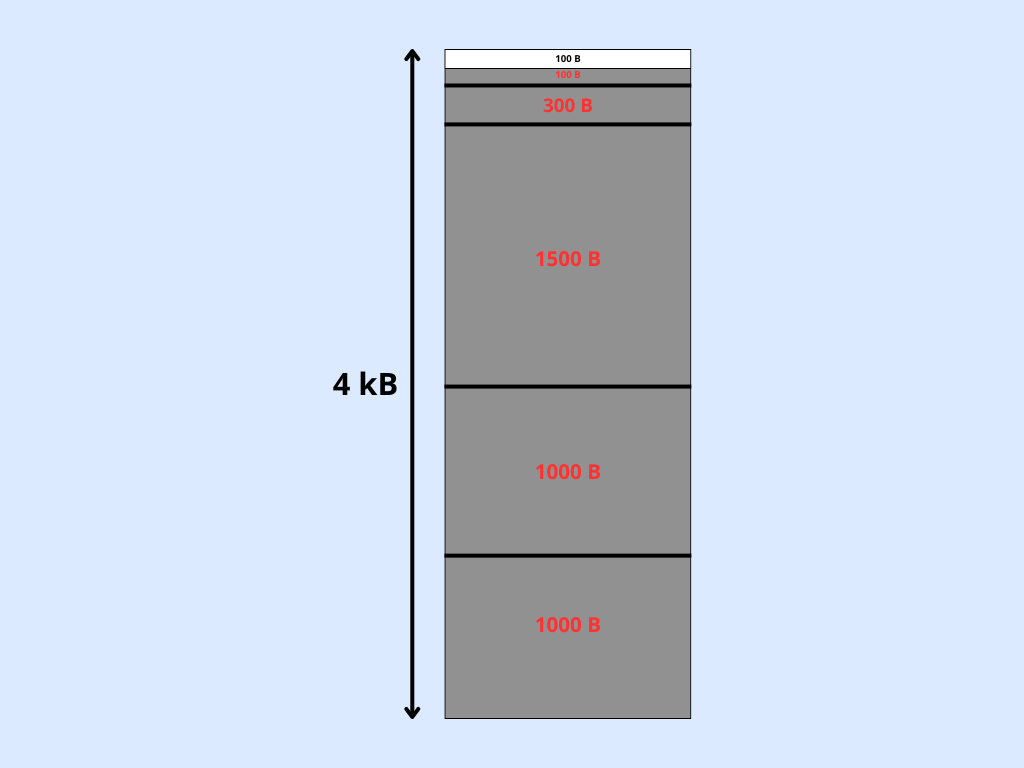
\includegraphics[width=0.65\linewidth]{img/best.png} 
    \vfill 
\end{frame}

\begin{frame}
    \centering
    {\Huge \textbf{Thanks for listening}}
\end{frame}

\end{document}
